The Neural Networks that we are using, and generally all the neural networks that estimate or generate something have an error rate, in our case, a missing rate from the real target. More specifically, our Neural Networks may falsie estimate some millimeter or centimeter from the real location of that keypoint. That may happen for each keypoint that they try to estimate for every frame. And every estimation is completely undependable from another. Therefore, this produces a type of noise through the motion data, that can be clearly seen even in our video mp4 player (for better visualization use Blender or another 3D computer graphics software tool-set). \\

The animators could reduce this noise by hand, correcting each joint location and orientation for each frame. This procedure is what is happening, even with mocap suits when the animators want to create flawlessly motion data. However, this procedure is clearly too time-consuming, since a video may contain over 1000 frames and each frame contains 17 joints with three or six dimensions each.\\

Therefore, we came up with a solution that will significantly reduce this noise. It may need some further editing from the animators, but we will save them again plenty of time. The best way to reduce the noise is to filter out with smoothing filter the motion data. We offer to the animators three different filters, the Mean, the Gaussian, and the Butterworth. \\

These filters are three well-known filters that many researchers use to reduce the noise from images. In our case, we want to remove the noise from the motion data. The form of the motion data is a 2D array, that has the same properties as an image. However, the fact that the motion data has the form of an image, is not the only reason that we can use these filters. It is that for every keypoint of the motion data, some of its neighbors have a dependence on it. For example, the keypoints of a bone have a dependence on their neighbor frames. This also happens in the images, every pixel has a dependent on some of its neighbors in order to create some shapes and objects.

\subsubsection*{Mean Filter}
Mean filtering \cite{Mean Filtering} is a simple, intuitive and easy to implement method of smoothing images, i.e. reducing the amount of intensity variation between one pixel and the next. It is often used to reduce noise in images. So we decided to use this to filter the noise from the motion data, imagine that each frame has a similar form of an image, however it is more sensitive to the noise.\\

The idea of mean filtering is simply to replace each pixel value in an image with the mean ('average') value of its neighbors, including itself. This has the effect of eliminating pixel values which are unrepresentative of their surroundings. Mean filtering is usually thought of as a convolution filter. Like other convolutions it is based around a kernel, which represents the shape and size of the neighborhood to be sampled when calculating the mean. Often a 3x3 square kernel is used, as shown in the figure below, although larger kernels (e.g. 5x5 squares, it has to be an odd number) can be used for more severe smoothing. (Note that a small kernel can be applied more than once in order to produce a similar but not identical effect as a single pass with a large kernel.)


\begin{figure}[h]
	\centering
	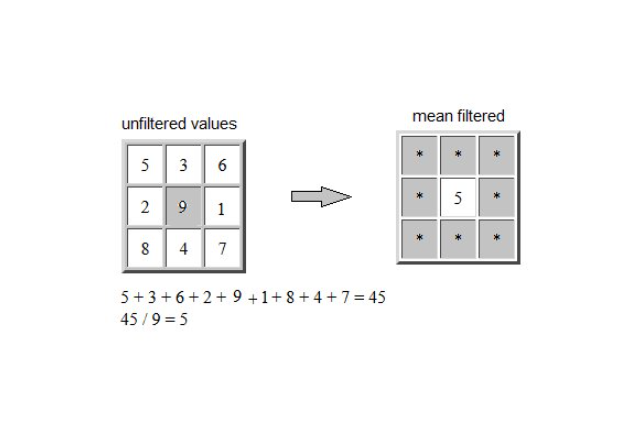
\includegraphics[width=1\textwidth]{figures/Implementation/meanFilter.png}
	\captionsetup{labelformat=empty}
	\caption{\href{https://www.researchgate.net/publication/348548607_The_Challenge_of_Predicting_OAG_Progression_from_the_Initial_Visual_Field_Test/figures?lo=1}
	{Mean Filter procedure with a 3x3 kernel}}
\end{figure}

In general, the Mean filter allows a great deal of high spatial frequency detail to pass while remaining very effective at removing noise on images where less than half of the pixels in a smoothing neighborhood have been effected. (As a consequence of this, mean filtering can be less effective at removing noise from images corrupted with Gaussian noise.)\\

One of the major problems with the mean filter is that it is relatively expensive and complex to compute. To find the mean it is necessary to sort all the values in the neighborhood into numerical order and this is relatively slow, even with fast sorting algorithms such as quicksort (it has an average complexity of O(log(N)) and in worst case O($N^2$)). The basic algorithm can, however,be enhanced somewhat for speed. A common technique is to notice that when the neighborhood window is slid across the image, many of the pixels in the window are the same from one step to the next, and the relative ordering of these with each other will obviously not have changed. Clever algorithms make use of this to improve performance.\\

In our algorithm, we ask the animator to give us the size of the kernel that he wants to use in order to filter the motion data. We suggest they use a kernel with a size smaller than 9x9, but they are free to use whatever they want that will increase the quality of the motion data and decrease their further editing on it.

\subsubsection*{Gaussian Filter}
The Gaussian smoothing operator is a 2-D convolution operator that is used to 'blur' images and remove detail and noise. In this sense it is similar to the mean filter, but it uses a different kernel that represents the shape of a Gaussian ('bell-shaped') hump. This kernel has some special properties which are detailed below.\\
The Gaussian distribution in 1-D has the form:
$$ G(x) = \dfrac{1}{\sqrt{2\pi\sigma}} e^{-\dfrac{(x-\mu)^2}{2\sigma^2}}$$

where $\sigma$ is the standard deviation of the distribution. We have also assumed that the distribution has a mean of zero (i.e. it is centered on the line x=0). 

\begin{figure}[h]
	\centering
	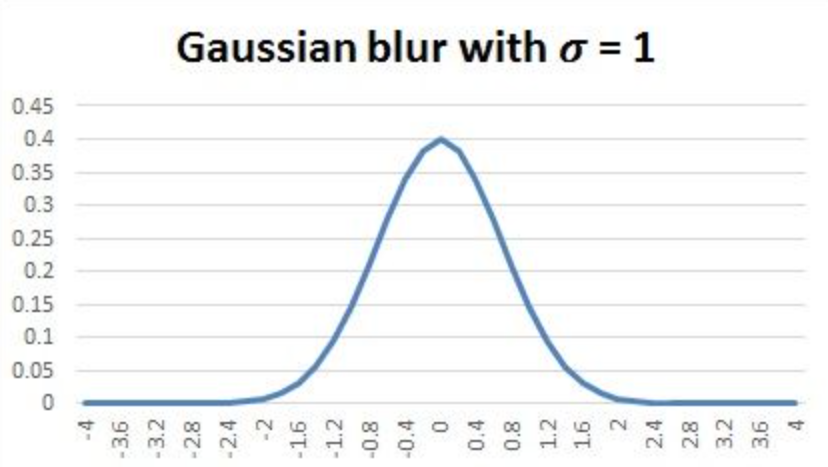
\includegraphics[width=1\textwidth]{figures/Implementation/Gaussian1D.png}
	\captionsetup{labelformat=empty}
	\caption{\href{https://fiveko.com/assets/pics/math/gauss1d_shape.jpg}
	{ 1-D Gaussian distribution with mean 0 and $\sigma$=1}}
\end{figure}

In our case we need a 2-D Gaussian Filter. Therefore, the idea of Gaussian smoothing is to use this 2-D distribution as a `point-spread' function, and this is achieved by convolution. Since the image is stored as a collection of discrete pixels we need to produce a discrete approximation to the Gaussian function before we can perform the convolution. In theory, the Gaussian distribution is non-zero everywhere, which would require an infinitely large convolution kernel, but in practice it is effectively zero more than about three standard deviations from the mean, and so we can truncate the kernel at this point. Figure 3 shows a suitable integer-valued convolution kernel that approximates a Gaussian with a $\sigma$ of 1.0. It is not obvious how to pick the values of the mask to approximate a Gaussian. One could use the value of the Gaussian at the centre of a pixel in the mask, but this is not accurate because the value of the Gaussian varies non-linearly across the pixel.\\

Once a suitable kernel has been calculated, then the Gaussian smoothing can be performed using standard convolution methods. The convolution can in fact be performed fairly quickly since the equation for the 2-D isotropic Gaussian shown above is separable into x and y components. Thus the 2-D convolution can be performed by first convolving with a 1-D Gaussian in the x direction, and then convolving with another 1-D Gaussian in the y direction. (The Gaussian is in fact the only completely circularly symmetric operator which can be decomposed in such a way.) \\



The Gaussian distribution in 2-D has the form:

$$ G(x,y) = \dfrac{1}{\sqrt{2\pi\sigma}} e^{-\dfrac{(x-\mu)^2 + (y-\mu)^2}{2\sigma^2}}$$\\

\pagebreak

\begin{figure}[h]
	\centering
	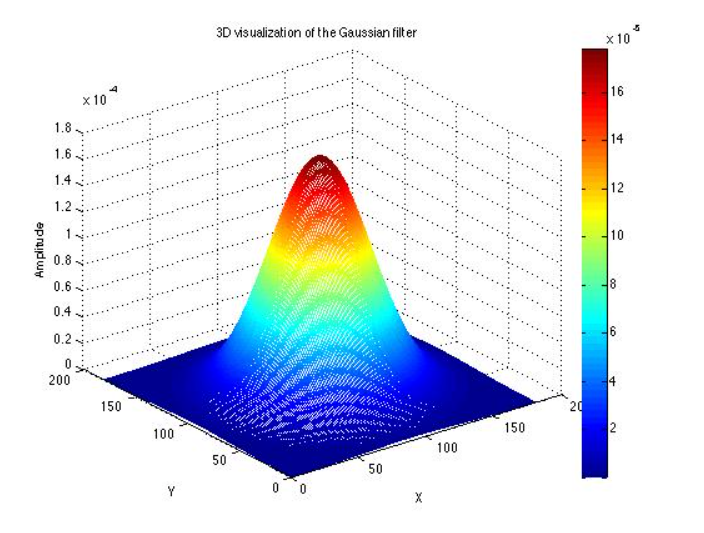
\includegraphics[width=1\textwidth]{figures/Implementation/Gaussian2D.png}
	\captionsetup{labelformat=empty}
	\caption{\href{https://stackoverflow.com/questions/23981437/visualization-of-gaussian-laplacian-etc-filters-in-matlab}
	{2-D Gaussian distribution with mean 0 and $\sigma$=1}}
\end{figure}

The effect of Gaussian smoothing is to blur an image, in a similar fashion to the mean filter. The degree of smoothing is determined by the standard deviation of the Gaussian. (Larger standard deviation Gaussian's, of course, require larger convolution kernels in order to be accurately represented.)\\

The Gaussian outputs a "weighted average" of each pixel's neighborhood, with the average weighted more towards the value of the central pixels. This is in contrast to the mean filter's uniformly weighted average. Because of this, a Gaussian provides gentler smoothing and preserves edges better than a similarly sized mean filter.\\

One of the principle justifications for using the Gaussian as a smoothing filter is due to its frequency response. Most convolution-based smoothing filters act as low-pass frequency filters. This means that their effect is to remove high spatial frequency components from an image. The frequency response of a convolution filter, i.e. its effect on different spatial frequencies, can be seen by taking the Fourier transform of the filter.\\

Both filters attenuate high frequencies more than low frequencies, but the mean filter exhibits oscillations in its frequency response. The Gaussian on the other hand shows no oscillations. In fact, the shape of the frequency response curve is itself (half a) Gaussian. So by choosing an appropriately sized Gaussian filter we can be fairly confident about what range of spatial frequencies are still present in the image after filtering, which is not the case of the mean filter. This has consequences for some edge detection techniques, as mentioned in the section on zero crossings. (The Gaussian filter also turns out to be very similar to the optimal smoothing filter for edge detection under the criteria used to derive the Canny edge detector.)\\

In our algorithm, we ask the animator to give us the standard deviation of the distribution, (the $\sigma$) as well as the border( the mean value $\mu$) in order to filter the motion data. Gaussian filter differs, what happens is to make each frame of the motion data less sharp and more united between the neighbor frames. Therefore, each motion data may have a unique ideal standard deviation of the distribution and border that the animators have to find by hand.

 
\subsubsection*{Butterworth Filter}
The first two filter were digital filters that many researchers use to clear the noise from images. We used them to clear the noise from the motion data, which works in our case due to some similarities that there are in images and our motion data. In this point, we propose another different type of filter that can also clear our motion data noise. \\

\begin{figure}[h]
	\centering
	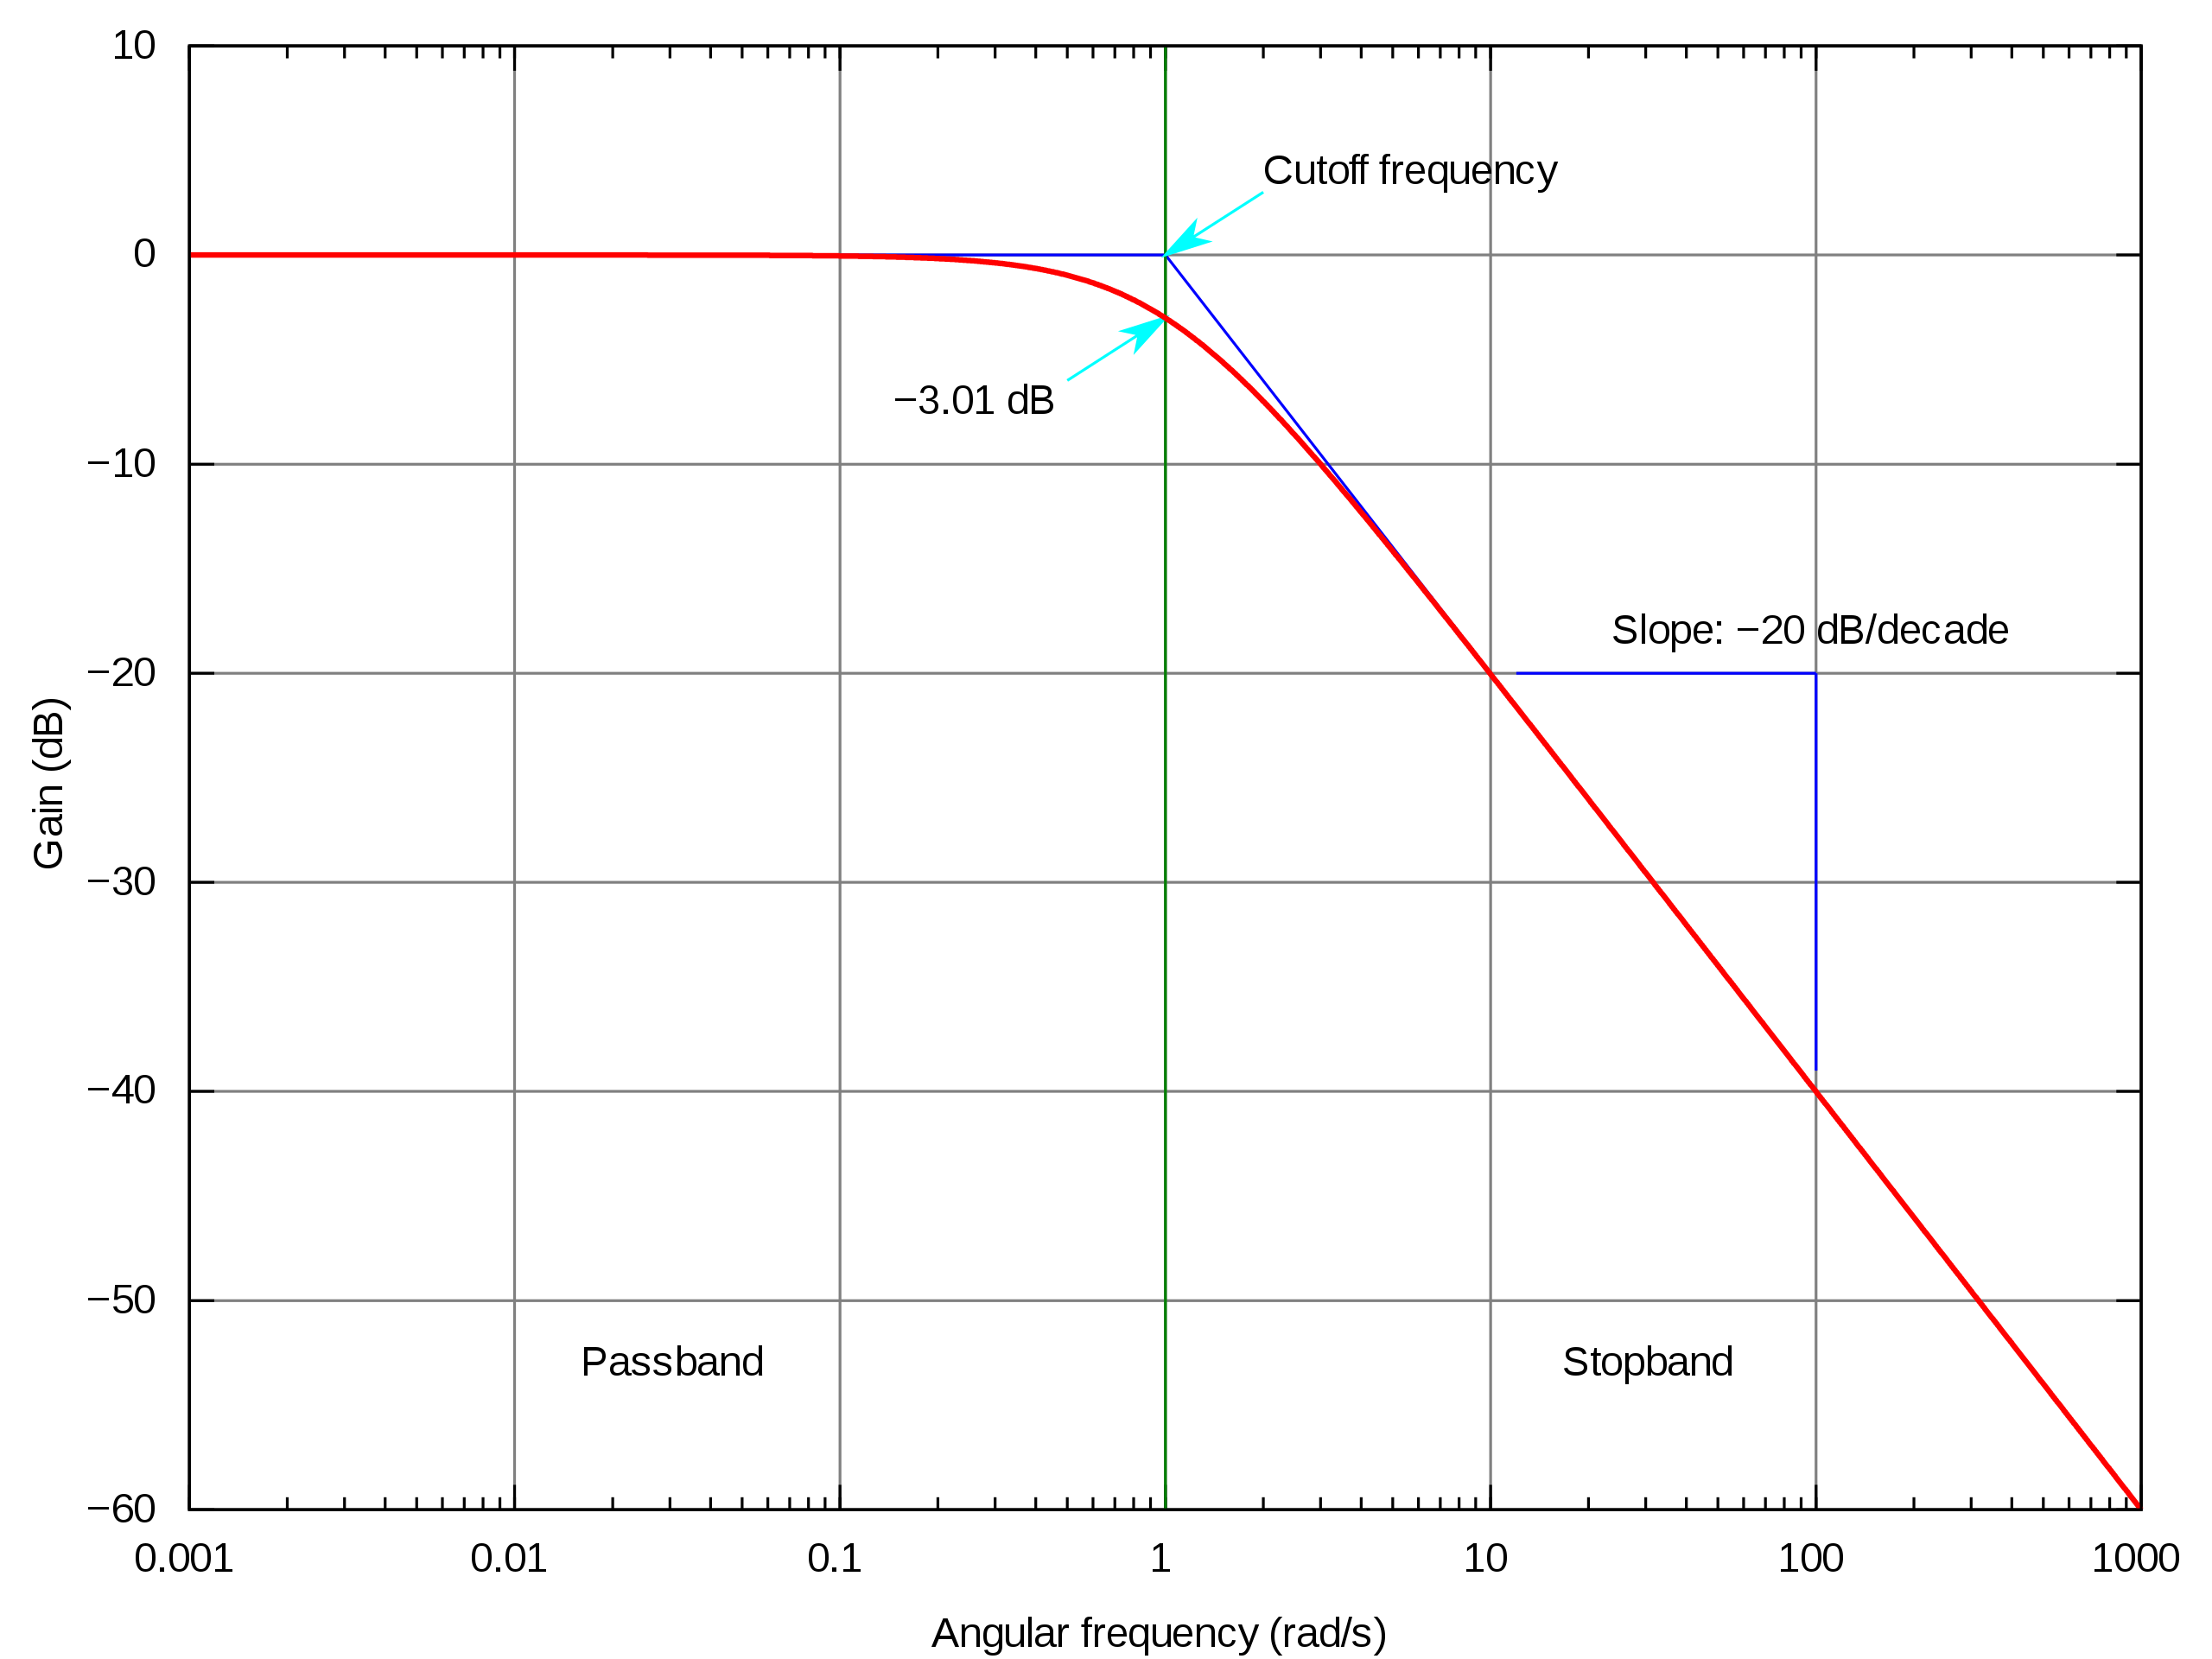
\includegraphics[width=0.7\textwidth]{figures/Implementation/butterworthfilter.png}
	\captionsetup{labelformat=empty}
	\caption{\href{https://upload.wikimedia.org/wikipedia/commons/thumb/6/60/Butterworth_response.svg/2560px-Butterworth_response.svg.png}
	{A low-pass Butterworth Filter}}
\end{figure}

The Butterworth filter is a type of signal processing filter designed to have as flat frequency
response as possible (no ripples) in the pass-band and zero roll off response in the stop-band.
Butterworth filters are one of the most commonly used digital filters in motion analysis and in
audio circuits. They are fast and simple to use. Since they are frequency-based, the effect of
filtering can be easily understood and predicted. Choosing a cutoff frequency is easier
than estimating the error involved in the raw data in the spline methods. However, one main
disadvantage of the Butterworth filter is that it achieves this pass band flatness at the expense
of a wide transition band as the filter changes from the pass band to the stop band. It also has
poor phase characteristics as well. The ideal frequency response, referred to as a "brick wall"
filter in the figure below.

\begin{figure}[h]
	\centering
	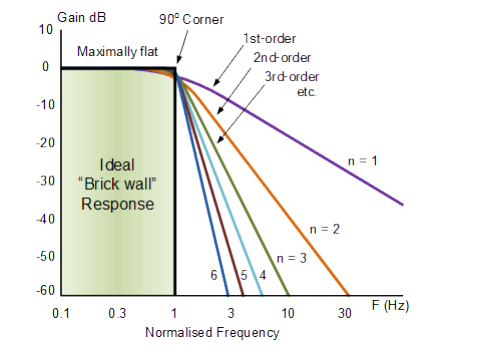
\includegraphics[width=1\textwidth]{figures/Implementation/butterworth.png}
	\captionsetup{labelformat=empty}
	\caption{\href{https://www.electronics-tutorials.ws/wp-content/uploads/2018/05/filter-fil57.gif}
	{Ideal Frequency Response for a low-pass Butterworth Filter}}
\end{figure}

The higher the Butterworth filter order, the higher the number of cascaded stages
there are within the filter design, and the closer the filter becomes to the ideal "brick wall"
response. However, in practice this "ideal" frequency response is unattainable as it produces
excessive pass-band ripple. The generalised equation representing a "nth" Order Butterworth filter, the frequency response is given as:

$$H_{(j\omega)} = \dfrac{1}{\sqrt{1 + \epsilon^2 (\dfrac{\omega}{\omega_p})^{2n}}}$$

Where: n represents the filter order, Omega $\omega$ is equal to $2\pi f$ and Epsilon $\epsilon$ is the maximum pass band gain, ($A_{max}$). If $A_{max}$ is defined at a frequency equal to the cut-off -3dB corner point ($f_c$), $\epsilon$ will then be equal to one and therefore $\epsilon^2$ will also be one. So we simplify the above equation, supposing that we have $A_{max}$ or $\dfrac{H_0}{H_1} = \sqrt{2}$ which means that the cut-off frequency is at -3dB, where $H_0$ is the Maximum Pass band Gain and $H_1$ the Minimum Pass band Gain.\\


In our algorithm, we ask the animator to give us the cut-off frequency , (the $\omega$), the order n of the butterworth filter as well as the fast Fourier transform  border in order to filter the motion data.\\

These are the three filters that we use to clean the noise from the motion data. To compare these filters someone must run the algorithm, since the output of the cleaning is a sequence of motion, and it is impossible to upload a video to represent it in this presentation. Nevertheless, all three of them can clean the majority of the noise that neural networks generate in the motion data, without affecting the motion information.